\documentclass[12pt]{article}

\usepackage{fontawesome}
\usepackage{hyperref}
\usepackage{xurl}
\usepackage{graphicx}
\usepackage{float}
\usepackage[tagged, highstructure]{accessibility}
\usepackage{bookmark}
\usepackage{enumitem}

\hypersetup{
    colorlinks=false,
    pdfborder={0 0 0},
    pdftitle={SQL Continued Lab},
    pdfauthor={Adrianna Holden-Gouveia},
    pdfsubject={Introduction to Data - Lab Assignment},
    pdflang={en-US},
    pdfkeywords={SQL, filters, functions, advanced queries, Khan Academy}
}

% Configure PDF bookmarks for navigation
\bookmarksetup{
    numbered,
    open,
}

% Configure list spacing for better accessibility
\setlist{nosep}



\title{SQL Continued}
\author{
        Adrianna Holden-Gouveia \\
        Website: \href{https://aholdengouveia.name}{aholdengouveia.name}\\ 
        \date{\vspace{-5ex}}
        %Email: \href{mailto:admin@aholdengouveia.name}{admin@aholdengouveia.name} \\
%        \faLinkedin{: aholdengouveia} \\
        \faGithub {: aholdengouveia} \\
        %\faTwitter {: aholdengouveia} \\
        }

%S\date{\today}


\begin{document}    

\maketitle

%\begin{abstract}
%This is a template for Linux Administration Lab work
%\end{abstract}
%\tableofcontents


\section*{Accessibility Notice}
This document is also available in HTML format at:

Link: \href{https://aholdengouveia.name/IntroData/labs/dbsql2.html}{\textbf{\nolinkurl{https://aholdengouveia.name/IntroData/labs/dbsql2.html}}}

The HTML version provides enhanced accessibility features including keyboard navigation, screen reader support, responsive design, dark mode support, and high contrast options.

\section*{Objectives:}
\begin{itemize}
    \item The objective of this lab is to continue working with SQL to learn more advanced topics such as filters and functions. Prior knowledge of SQL is assumed. Students will gain an understanding of SQL functions and filters through interactive methods utilizing a free online tutorial and other resources.
\end{itemize}
\section*{Lab Instructions}

References, a video, a PowerPoint and some notes are available at my website
Link: \href{https://www.aholdengouveia.name/IntroData/sql2.html}{\textbf{\nolinkurl{https://www.aholdengouveia.name/IntroData/sql2.html}}}

The tutorial you will be following is here: Link: \href{https://www.khanacademy.org/computing/computer-programming/sql/more-advanced-sql-queries/pt/more-complex-queries-with-andor}{\textbf{\nolinkurl{https://www.khanacademy.org/computing/computer-programming/sql/more-advanced-sql-queries/pt/more-complex-queries-with-andor}}} 


\subsection*{Questions}
    \begin{enumerate}
        \item How do you think this tutorial compares to the first Khan Academy tutorial you did in the SQL 1 lab? Why?
        \item What do you think is missing from this tutorial? Why?
        \item For \textbf{each} of the 4 challenges and the final project (5 total), include:
        \begin{enumerate}
            \item The name of the challenge or project
            \item A screenshot of your answer
            \item What, if anything, you found challenging, and why
        \end{enumerate}
        The 4 challenges are Karaoke song selector, Playlist maker, The wordiest author, and Gradebook. The final project is Data dig.
    \end{enumerate}

\textbf{Screenshot rules:} make sure to have a note with your name and the term in each screenshot. The screenshot should be focused on the note and your answer, not the full desktop.  Any screenshots that don't include the note, or are full desktop, or taken with a camera instead of a screenshot won't count and will earn no points. This is an example of what it should look like:

        \begin{figure}[H]
            \centerline{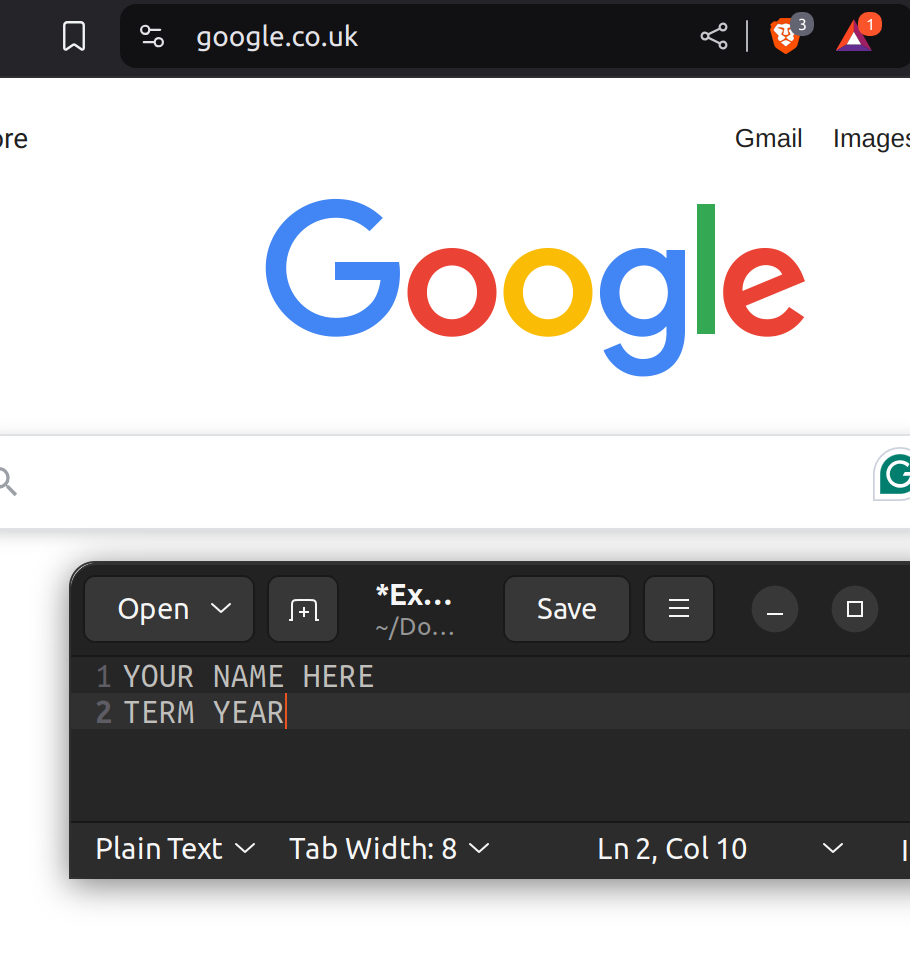
\includegraphics[scale=.2]{ExampleScreenshot.png}}
            \caption{This is an image of what each of your screenshots should look like}
            \alt{Example screenshot: a web browser showing the Google home page, with a small text editor window in front of it that says YOUR NAME HERE and TERM YEAR}
            \end{figure}

    \section*{Tutorial Recommendation}
You will find 3 tutorials for someone who wants to learn SQL filters and functions, compare them, and then write a more thorough review of your favorite.  The tutorials can be interactive or not.  Videos that you can follow along with count as tutorials for this.

\textbf{Everything you list must be new.} You must find these yourself:
\begin{itemize}
    \item Do not ask an AI to find or recommend them.
    \item Do not include anything I've shared on Brightspace or my website.
    \item Do not include anything you've already submitted for another assignment.
\end{itemize}

\subsection*{Part 1: Compare 3 tutorials}
Find 3 tutorials or videos on SQL filters and functions. For \textbf{each} one, include:
\begin{enumerate}[label=(\alph*)]
    \item Its title and link
    \item Its type (interactive, video, or written)
    \item Its pros
    \item Its cons
\end{enumerate}

\subsection*{Part 2: Review your favorite}
Pick your favorite of the 3 and write a more thorough review of it. Your review should include:
\begin{enumerate}[label=(\alph*)]
    \item Why you picked it over the other two
    \item What it covers
    \item How well it teaches SQL filters and functions
    \item What, if anything, is missing or could be better
    \item Who you would recommend it to
\end{enumerate}

Your review should be at least one paragraph and no more than two pages.

\section*{Deliverables}
You may submit everything in one document, or in two documents where the second one is your Tutorial Recommendation.
\begin{enumerate}
    \item Your answers to questions 1 to 3, labelled with their question numbers
    \item All 5 screenshots, following the screenshot rules
    \item Your Tutorial Recommendation: Part 1 (comparing 3 tutorials) and Part 2 (the review of your favorite)
\end{enumerate}
\end{document}